\chapter{CUORE}

CUORE (Cryogenic Underground Observatory for Rare Events) is located in Gran Sasso, Italy, and utilizes a bolometric method to search for \zeronubb. The experiment will run with 988 crystals of TeO$_2$ held at roughly 10 mK.
The source of \zeronubb~are the $^{130}$Te nuclei inside of the crystals ($34.2\%$ natural abundance \cite{Fehr200483}).
Thus, in this setup, the crystals act as both sources and detectors of \zeronubb. When energy is deposited in the crystals, such as from the electrons emitted during \zeronubb, the temperature of the crystals rises.
The Q-value of the decay of interest, viz. $^{130}\textrm{Te} \rightarrow ^{130}\textrm{Xe} + e + e$, is $2527.518\pm 0.013$ keV \cite{Redshaw:2009cf, Scielzo:2009nh, Rahaman:2011zz}.
This high Q-value is well-separated from other naturally occurring environmental $\gamma$'s except for $^{60}$Co at 2506 keV and $^{208}$Tl at 2615 keV.
However, the resolution of the CUORE crystals is $7.7\pm0.5$ keV, which means that these peaks do not significantly worsen the background in the region of interest at the Q-value.
In addition, this resolution aids in understanding background sources that deposit energy the detector as each \gamma~line can be observed above the Compton background, which aids in identifying particular background sources.

\section{CUORE Detectors}

\subsection{Particle Detection with Bolometers}
As noted in \autoref{sec:State of Neutrinoless Double Beta Decay Experiments}, current experiments in the field of \zeronubb~use a wide array of technologies to identify \zeronubb~events.
However, CUORE utilizes a different method of calorimetry than its counterparts in that it uses a technique known as the bolometric method.
As particles pass through matter, the energy they deposit is eventually carried into the surrounding material as heat.
This method requires a mass that acts as a thermal capacitor, a weak thermal connection to a heat bath, and a thermometer (generally a thermistor) and CUORE's setup is sketched in \autoref{fig:thermal_crystal_cartoon} and a sample pulse is shown in \autoref{fig:Sample_pulse}. The detectors in CUORE, $\textrm{TeO}_2$~crystals, respond to energy deposition by a temperature rise according to
\begin{equation}
\delta T = \delta E/C(T).
\end{equation}
At low C, $\delta T$ is maximized; therefore, the crystals are operated at low temperatures where C(T) is given by the Debye Model:
\begin{equation}
C(T)\sim (\frac{T}{\Theta_D})^3
\end{equation} 
where $\Theta_D$ is the Debye temperature for \teotwo, $232\pm7~\textrm{K}$ \cite{BolometerCalculations}. This strong temperature dependence on the heat capacity is what drives the need for low temperatures in CUORE, where we have achieved an operational temperature of $\sim10$ mK.
The custom cryostat used to do this is described later on in \autoref{sec:CUORE Cryostat}.
At these temperatures, a 1 MeV energy deposit in a single CUORE crystal would cause the temperature to rise to $\sim 100~\textrm{\mu K}$. 

\begin{figure}[htbp]
\centering
\includegraphics[width=0.7\linewidth]{Figures/bolosketch-color.pdf}
\caption[A diagram of the thermal connection of the TeO$_2$ crystals to the thermal bath provided by the copper frames.]
{A diagram (not to scale) of the thermal connection of the TeO$_2$ crystals to the thermal bath provided by the copper frames.
The weak thermal coupling is provided by the PTFE.}
\label{fig:thermal_crystal_cartoon}
\end{figure}

\begin{figure}[htbp]
\centering
\includegraphics[width=0.7\linewidth]{Figures/pulse-conference.pdf}
\caption[An example pulse from a single CUORE detector.]
{An example pulse from a single CUORE detector.
After an event at 1 s where energy is deposited in the crystal, a fast temperature rise is observed along with a slow cooling through the weak coupling to the thermal bath.}
\label{fig:Sample_pulse}
\end{figure}

Of course, an integral component to the bolometric method is the choice of thermometer used to detect these changes in temperature.
The choice of thermometer that CUORE uses is a Neutron Transmutation Doped (NTD) germanium thermistor due to its reproducibility and uniformity, which is critically important across CUORE's crystal array. However, a drawback to this is that each NTD thermistor must be individually cut from a block and then mounted onto each bolometer \cite{NTDThermistor}.
The NTD thermistorks works under the principle of causes the conduction electrons to localize into the doped atoms which are spread out into the germanium.
At high temperatures, the electrons tunnel to the nearest available unoccupied sites.
At low temperatures such as the $<1~K$ temperatures of CUORE, the resulting lack of higher-energy phonons prevents the electron from tunneling into the nearest sites, and instead favor sites with similar energies to the electron.
In this regime of ``variable range hopping", the resistance of the NTD goes as
\begin{equation}
    R(T) = R_0 e^{\left(\frac{T_0}{T}\right)^p} 
    \label{eq:NTD_Resistivity}
\end{equation}
as shown by Shklovskii and Efros \cite{NTDResistivity}.
This causes the resistivity to have a strong temperature dependence at cryogenic temperature and allows the NTD thermistor to serve as the thermometer to measure the temperature rise as a voltage, as shown in \autoref{fig:Sample_pulse}.

\subsection{CUORE Detector Array}
CUORE uses 988 \teotwo~crystals as bolometers arranged in 19 towers with 13 floors as shown in \autoref{fig:cuore_detector_array}.
These crystals are $5\times5\times5~\textrm{cm}^3$ in size and have mass 750g each, for a total of 742 kg of \teotwo.
Taking advantage of the relatively high natural isotopic abundance of Te, shown in \autoref{fig:q_vs_ia-color}, this comes to a total mass of 206 kg of $^{130}$Te and 189 kg of $^{128}$Te.
Each tower is approximately 80 cm tall, such that in operation, these crystals form the coldest cubic meter in the known universe \cite{Ouellet:2014qua}.

\begin{figure}
    \centering
    \includegraphics[width=0.8\linewidth]{Figures/CUORE_detector_array_0.png}
    \caption[A schematic of the CUORE detector array.]
    {A schematic of the CUORE detector array.
    The detectors are held in place by the copper frames and arranged in 19 towers with 13 floors each.}
    \label{fig:cuore_detector_array}
\end{figure}

\begin{figure}
    \centering
    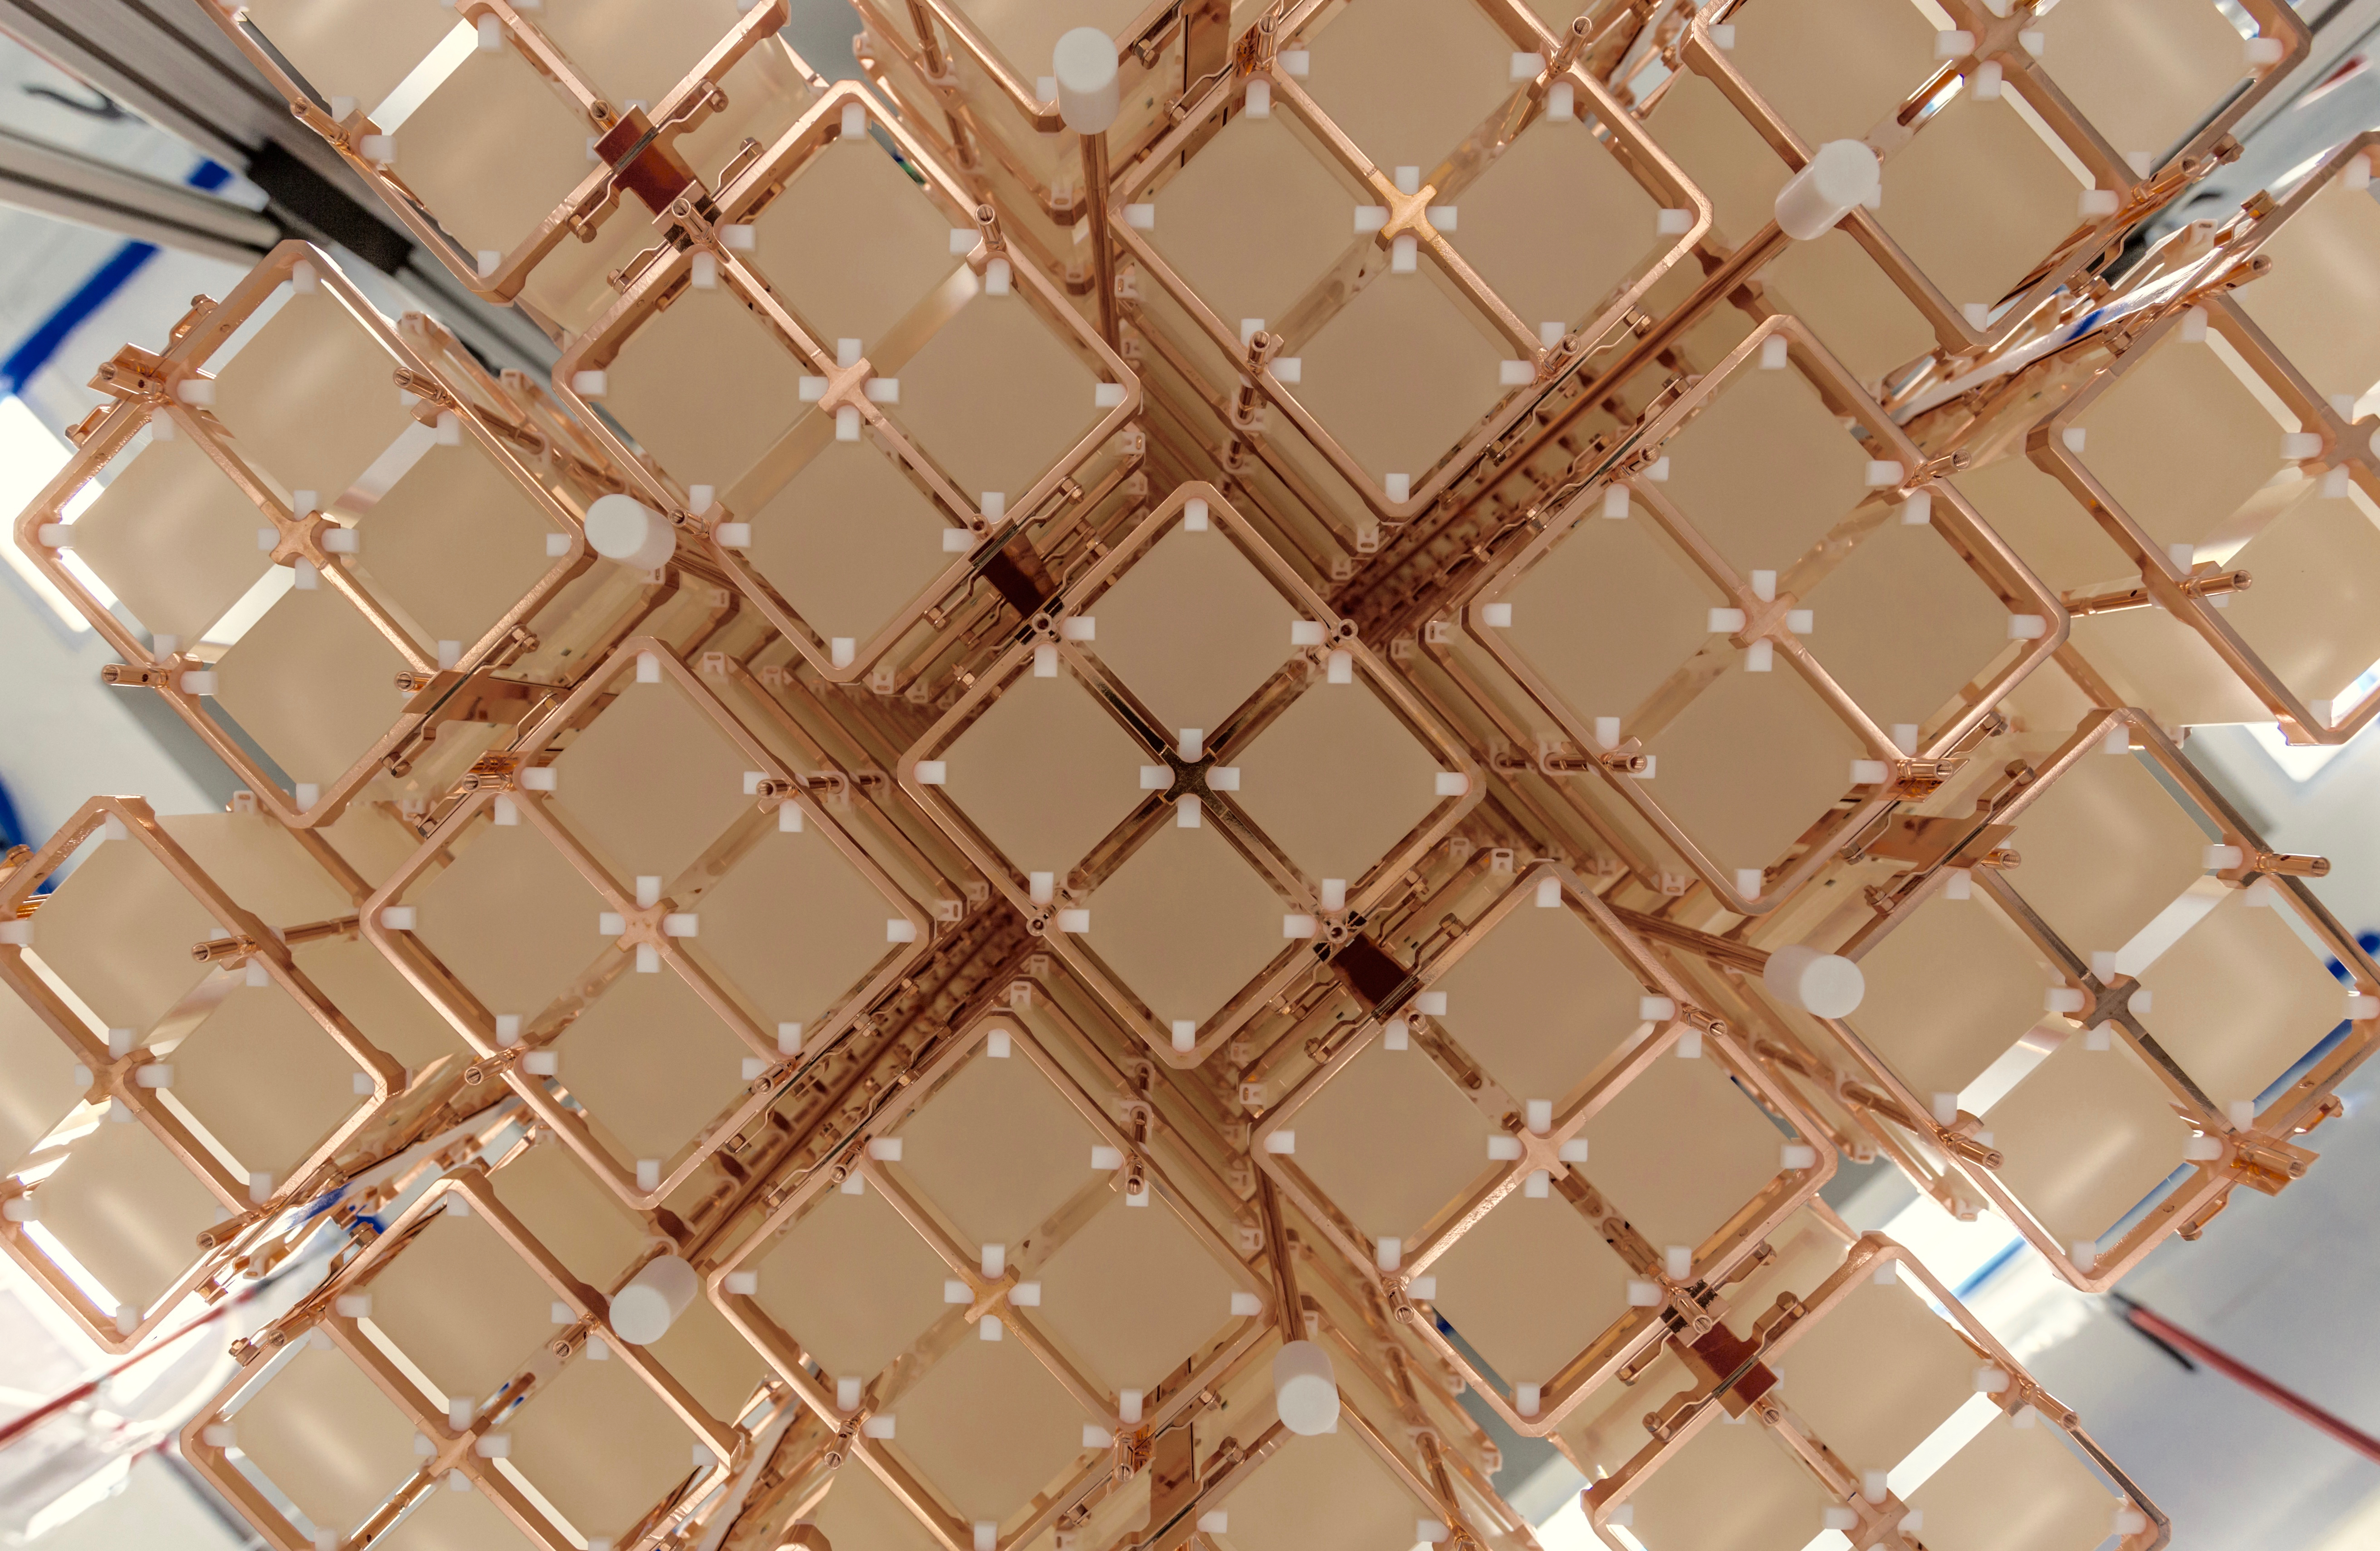
\includegraphics[width=0.8\linewidth]{Figures/CUORE_29Aug16_HR-2477.jpg}
    \caption[A photograph of the 19 CUORE towers from below.
    Photo Credit: Yury Suvorov.]
    {A photograph of the 19 CUORE towers from below after installation in the cryostat.
    Also visible are the inner calibration source tubes with their teflon caps.
    Photo Credit: Yury Suvorov.}
    \label{fig:my_label}
\end{figure}

\section{Predecessor Experiments}
The CUORE experiment benefits from the experience gained through multiple previous incarnations of this bolometric technique in \teotwo.
Starting with the smallest proof-of-concept detectors, successive generations of this technology have increased in total detector mass and decreased in background in order to increase sensitivity and further probe \zeronubb~decay.
This almost-exponential growth in mass in the different generations of CUORE-like experiments from 73~g to 742~kg is shown in \autoref{fig:bolometer_mass_over_time}.
Of course, as shown in \autoref{eq:sensitivity_short}, the detector mass is only one part of the sensitivity equation, but successive experiments have also significantly reduced backgrounds and other improvements to increase sensitivity beyond merely the increase from increased mass. 
\begin{figure}[htbp]
    \centering
    \includegraphics[width=\linewidth]{Figures/bolometer_mass_over_time.pdf}
    \caption[The increase in mass of \teotwo~crystals in successive experiments.]
    {The increase in mass of \teotwo~crystals in successive experiments.}
    \label{fig:bolometer_mass_over_time}
\end{figure}
\subsection{Cuoricino}

\subsection{CUORE-0}
After the completion of the Cuoricino experiment, an intermediate experiment was planned while working on completing the CUORE cryostat.
This experiment, CUORE-0, was meant to bridge the gap between the two experiments with a single CUORE-like tower placed in the Cuoricino cryostat.
A schematic of the experimental apparatus can be seen in \autoref{fig:CUORE-0_cryostat_schematic}.

\begin{figure} [htbp]
    \centering
    \includegraphics[width=0.8\linewidth]{Figures/CUORE-0_cryostat_schematic.pdf}
    \caption[A schematic of the CUORE-0 experiment.]
    {A schematic of the CUORE-0 experiment in the Cuoricino cryostat (not to scale).
    The CUORE-0 tower is in the center of the cryostat, and the calibration sources are deployed between the OVC and the external lead shield.}
    \label{fig:CUORE-0_cryostat_schematic}
\end{figure}

The purpose of this experiment, besides  making a measurement of \zeronubb, was to validate the improved materials selection and cleaning of the CUORE crystals.
This improvement is quantified in \autoref{fig:cuore-0_vs_cuoricino} where a signficant decease is observed in the \alpha~backgrounds which are due to components nearest to the crystals.
The \gamma~backgrounds are not reduced as significantly as the cryostat is the same between the CUORE and Cuoricino experiments.

\begin{figure}[htpb]
    \centering
    \includegraphics[width=\linewidth]{Figures/CUORE-0_vs_Cuoricino.pdf}
    \caption[A comparison of the backgrounds in the Cuoricino and CUORE-0 exeperiments.]
    {A comparison of the backgrounds in the Cuoricino and CUORE-0 experiments.
    The backgrounds are significantly reduced in the \gamma~ regions as the improved materials selection and cleaning procedures reduced the surface contaminants on the \teotwo~crystals and the copper frames on the tower.
    There is also some improvement on the level of \gamma~ backgrounds, but as the cryostat is the same, those contaminations remain.
    However, one peak in the \alpha region from $^{210}$Po does not decrease, and may be particular to this single tower.}
    \label{fig:cuore-0_vs_cuoricino}
\end{figure}

CUORE-0 collected data between 2013 and 2015, and during this time, many analysis and data-collection techniques were refined and improved for use in CUORE.
In particular, from the data collected, CUORE-0 was able to make the most precise measurement of \twonubb~decay in $^{130}$Te at the time, listed in \autoref{tab:2nuHalfLife} \cite{Alduino:2016vtd}.
In addition, CUORE-0 also performed a search for \zeronubb~and, in a combined analysis with the Cuoricino experiment, formed the most stringent limit at the time for \zeronubb~decay in $^{130}$Te with a limit of $T^{0ν}_{1/2}>4.0\times10^{24}$ yr \cite{Alfonso:2015wka}.

\section{CUORE Cryostat}
\label{sec:CUORE Cryostat}

Since the heat capacity of the CUORE crystals is so strongly dependent on temperature, it is important to have a system that can cool down the crystals to low temperatures and keep them running in stable conditions over long periods.
To this end, we constructed a cryogen-free custom cryostat to house the crystals.
The cooling components of the cryostat are pulse tubes that cools the cryostat stages at 40 K and 4 K and a dilution refrigerator that is responsible for maintaining the coldest regions of the cryostat, including the crystals at 10 mK.
In addition to cooling the crystals, the cryostat also houses the shielding for the crystals and, since this is a low-background experiment, needs to be made of radiopure materials, especially near the detectors themselves.

\begin{figure}[htbp]
\centering
\includegraphics[width=\linewidth]{Figures/cryostat_Adjusted.png}
\caption[CAD cutaway of the CUORE cryostat.]
{A CAD drawing of a cutaway the CUORE cryostat showing the internal shielding of the cryostat.
The temperature stages of the cryostat are also shown.
Not included are the external shields which extend around the sides of the cryostat.}
\label{fig:cryostat_cad_cutout}
\end{figure}

\subsubsection*{Cooling Systems}
\label{sssec:Cooling Systems}
One of the main cryostat changes between the previous experiments of CUORE-0 and CUORE was the change to a cryogen-free cryostat that uses pulse tubes instead of an external supply of liquid nitrogen, helium, and a 1~K bath.
This change allows for increased live-time of the experiment as data-taking does not need to be interrupted by the need to refill the bath.
However, this does come at a cost of increased mechanical noise as the 5 pulse tubes in CUORE input mechanical vibrations onto the cryostat.
In addition, since the 5 pulse tubes on CUORE are not symmetrically aligned due to space constraints, it is nontrivial to find a phase configuration that minimizes the noise, requiring an in-depth scan of varying pulse tube phases to find when the mechanical noise induced by the pulse tubes is minimized over the detectors.
Since the cyrostat needs to reach temperatures of 10 mK, a dilution refrigerator is used as the main cooling mechanism in the coldest stages of the cryostat.
A dilution refrigerator works by taking advantage of the phase boundary between dilute and concentrated phases of a $^3$He and $^4$He mixture, shown in \autoref{fig:He_phase_diagram}.
In the mixing chamber of the dilution refrigerator on the 100~mK stage of the CUORE cryostat, $^3$He flows from the concentrated phase to the dilute phase.
This process extracts energy from the environment of the mixing chamber, and by extension the coldest stages of the cryostat, as energy is required to move the $^3$He across the phase boundary\footnote{Of course, the Universe's entropy is not reduced by this exchange and additional energy is used to induce this endothermic cooling.}.

\begin{figure}
    \centering
    \includegraphics[width=0.6\linewidth]{Figures/Helium_phase_diagram.pdf}
    \caption[Phase diagram for $^{3}$He and superfluid $^{4}$He.]
    {Phase diagram for $^{3}$He and superfluid $^{4}$He.
    The separation between the dilute and concentrated phases provides the power that cools the cryostat down to mK-scale temperatures.}
    \label{fig:He_phase_diagram}
\end{figure}

\begin{table}[htbp]
    \centering
    \begin{tabular}{c|c}
    \hline
    \hline
    Thermal Stage     & Cooling Power  \\
    \hline
    40~K     & 1~W \\
    4~K      & 300~mW \\
    600~mK   & 550~$\mu$W \\
    50~mK    & 1.1~$\mu$W \\
    10~mK    & 1.2~$\mu$W \\
    \hline
    \hline
    \end{tabular}
    \caption[The cooling power of the cryostat at varying thermal stages.]
    {The cooling power of the cryostat at varying thermal stages.
    The power is maximized in warmer stages, but decreases significantly towards the coldest stages.
    \color{red}Check these \#s with Vivek \color{black}}
    \label{tab:cryostat_cooling_power}
\end{table}
\subsubsection*{Radiopurity}

\begin{figure}[htbp]
\centering
\includegraphics[width=0.7\linewidth]{Figures/CUORE_background_budget}
\caption[CUORE background budget.]
{CUORE background budget.
The CUORE goal is 0.01 counts/keV/kg/y with most of the background due to the surfaces of cryostat elements nearest to the crystal and the bulk of the Roman lead.}
\label{fig:cuore_background_budget}
\end{figure}

The background goal of CUORE is to have no greater than 0.01 counts/keV/kg/yr in the region of interest, defined to be a 100 keV interval from 2470 keV to 2570 keV. In order to achieve this low background, the parts nearest to the detectors undergo intensive cleaning. The contamination of these surfaces is given in \autoref*{tab:NearDetectorSources}.

\begin{table}[htbp]
\centering
\caption[90\% upper limits of $^{232}$Th and $^{238}$U bulk contamination of sources near the detector.]
{90\% upper limits of $^{232}$Th and $^{238}$U bulk contamination of sources near the detector.
The units in the table are relative masses of contamination to the mass of the component.
Table from \cite{Alduino:2016vjd}}
\label{tab:NearDetectorSources}.
\begin{tabular}{|c|c|c|}
\hline 
 Component & $^{232}$Th [g/g] & $^{238}$ U [g/g] \\ 
\hline 
TeO$_2$ crystals & $< 2.1\times 10^{-13}$ & $<5.3\times 10^{-14}$ \\ 
\hline 
NOSV copper & $<5.0 \times 10^{-13}$ & $<5.3 \times 10^{-12}$ \\ 
\hline 
NTD sensors & $< 1.0 \times 10^{-9}$ & $<1.0 \times 10^{-9}$ \\ 
\hline 
Bonding gold wires & $< 1.0 \times 10^{-8}$ & $<1.0 \times 10^{-9}$ \\ 
\hline 
Si heaters &   $<8\times 10^{-11}$ & $<1.7 \times 10^{-10}$ \\ 
\hline 
PTFE holders & $<1.5\times 10^{-12}$ & $<1.8 \times 10^{-12}$ \\ 
\hline 
Cu-PEN cables & $<4.4\times 10^{-10}$ & $<1.1 \times 10^{-10}$ \\ 
\hline
Glue & $<2.2\times 10^{-10}$ & $<8.2\times10^{-10}$ \\
\hline 
\end{tabular} 
\end{table}



\begin{comment}

\subsection{CUORE Detectors}

The CUORE detectors are 988 $ 5\times 5 \times 5~ \textrm{cm}^3$ crystals arranged into 19 towers with 13 floors containing 4 crystals each as shown in \hyperref[fig:cuore-detector-array0]{Fig. \ref*{fig:cuore-detector-array0}}. The total detector mass is 742 kg with 206 kg of $^{130}$Te. 

\begin{figure}[htbp]
\centering
\includegraphics[width=0.7\linewidth]{"Figures/CUORE detector array_0"}
\caption{A rendering of the CUORE towers. The 19 towers are arranged into rows of 3, 4, 5, 4, and 3 towers.}
\label{fig:cuore-detector-array0}
\end{figure}


The crystals in each tower are held by copper frames, with polytetrafluoroethylene (PTFE) in between the copper and the crystals. The crystals respond to energy deposition by a small temperature rise according to
\begin{equation}
\delta T = E/C(T).
\end{equation}
At low C, $\delta T$ is maximized; therefore, the crystals are operated at low temperatures where C(T) is given by the Debye Model:
\begin{equation}
C(T)\sim T^3.
\end{equation}
At 10 mK, the operating temperature of CUORE, the heat capacity is $\sim2$ nJ/K, which causes a 1 MeV energy deposit to have a $\delta T$ of $\sim0.1$ mK.

This temperature rise is measured by a neutron-transmutation-doped (NTD) germanium thermistors which are glued onto each crystal. These thermistors allow the temperature change of the crystals to be read out by electronics as a change in applied voltage. Also glued on the crystals are silicon resistors which are used as a Joule heater. Bonded to the thermistors and the heaters are gold wires which are bonded to copper tape with a polyethylene naphthalate (PEN) substrate (collectively called Cu-PEN) on wire trays along the sides of the towers, shown in \hyperref[fig:bondedchips]{Fig. \ref*{fig:bondedchips}}.
\begin{figure}[htbp]
\centering
\includegraphics[width=0.7\linewidth]{Figures/BondedChips}
\caption{A germanium NTD on the crystal with four gold wires that have been bonded to both the NTD and to copper pads on the Cu-PEN tape.}
\label{fig:bondedchips}
\end{figure}
These signals are then read out by room-temperature electronics on top of the cryostat. A rendering of a full tower with the copper frames, wire trays, PTFE, and crystals can be seen at \hyperref[fig:SingleTowerWithZoom]{Fig. \ref*{fig:SingleTowerWithZoom}}

\begin{figure}[htbp]
\centering
\includegraphics[width=0.7\linewidth]{Figures/C0TowerZoom.pdf}
\caption[A rendering of a single tower in the CUORE detector assembly with a cutout for a single floor. Adjacent floors share the same frames.]{A rendering of a single tower in the CUORE detector assembly with a cutout for a single floor. Adjacent floors share the same frames. Diagram from \cite{Alduino:2016vjd}}
\label{fig:SingleTowerWithZoom}
\end{figure}

After an energy deposition causes the temperature of the crystal to rise, the crystal returns slowly back to the baseline temperature due to the weak thermal connection between the crystals and the copper frames which are held at 10 mK. A diagram of the thermal connection is shown in \hyperref[fig:thermal_crystal_cartoon]{Fig. \ref*{fig:thermal_crystal_cartoon}}. The rise and fall times of the signal are around 0.05 seconds and 0.2 seconds, respectively, for a 2615 keV signal.

\begin{figure}[htbp]
\centering
\includegraphics[width=0.7\linewidth]{Figures/BolDetector_Cartoon.pdf}
\caption[A diagram of the thermal connection of the TeO$_2$ crystals to the thermal bath provided by the copper frames. The weak thermal coupling is provided by the PTFE and the gold wires for the NTD and the heater. The thermistor is not shown to scale.]{A diagram of the thermal connection of the TeO$_2$ crystals to the thermal bath provided by the copper frames. The weak thermal coupling is provided by the PTFE and the gold wires for the NTD and the heater. The thermistor is not shown to scale. Diagram from \cite{Alduino:2016vjd}}
\label{fig:thermal_crystal_cartoon}
\end{figure}

\subsection{CUORE Cryostat}

Since the heat capacity of the CUORE crystals is so strongly dependent on temperature, it is important to have a system that can cool down the crystals to low temperatures and keep them running in stable conditions over long periods. To this end, we constructed a custom cryostat to house the crystals. The cooling components of the cryostat are pulse tubes that cools the cryostat stages held 4 K, and a dilution refrigerator that is responsible for maintaining the coldest regions of the cryostat, including the crystals at 10 mK. In addition to cooling the crystals, the cryostat also houses the shielding for the crystals and needs to be made of radiopure materials, especially near the detectors themselves.

\begin{figure}[htbp]
\centering
\includegraphics[width=\linewidth]{Figures/Cryostat_Adjusted.png}
\caption{A CAD drawing of a cutaway the CUORE cryostat showing the internal shielding of the cryostat. The temperature stages of the cryostat are also shown. Not included are the external shields which extend around the sides of the cryostat}
\label{fig:cryostat_cad_cutout}
\end{figure}

\subsubsection*{Cooling Systems}

Since the cyrostat needs to reach temperatures of 10 mK, a dilution refrigerator is used as the main cooling mechanism in the coldest stages of the cryostat. A dilution refrigerator works by diluting a He-3 solution
%The CUORE cryostat 

\subsubsection*{Radiopurity}

\begin{figure}[htbp]
\centering
\includegraphics[width=0.7\linewidth]{Figures/CUORE_background_budget}
\caption{CUORE background budget. The CUORE goal is 0.01 counts/keV/kg/y with most of the background due to the surfaces of cryostat elements nearest to the crystal and the bulk of the Roman lead.}
\label{fig:istogramma}
\end{figure}

The background goal of CUORE is to have no greater than 0.01 counts/keV/kg/yr in the region of interest, defined to be a 100 keV interval from 2470 keV to 2570 keV. In order to achieve this low background, the parts nearest to the detectors undergo intensive cleaning. The contamination of these surfaces is given in \hyperref[tab:NearDetectorSources]{Table \ref*{tab:NearDetectorSources}}.

\begin{table}[htbp]
\centering
\caption[90\% upper limits of $^{232}$Th and $^{238}$U bulk contamination of sources near the detector.]{90\% upper limits of $^{232}$Th and $^{238}$U bulk contamination of sources near the detector. Table from \cite{Alduino:2016vjd}}
\label{tab:NearDetectorSources}
\begin{tabular}{|c|c|c|}
\hline 
 Component & $^{232}$Th [g/g] & $^{238}$ U [g/g] \\ 
\hline 
TeO$_2$ crystals & $< 2.1\times 10^{-13}$ & $<5.3\times 10^{-14}$ \\ 
\hline 
NOSV copper & $<5.0 \times 10^{-13}$ & $<5.3 \times 10^{-12}$ \\ 
\hline 
NTD sensors & $< 1.0 \times 10^{-9}$ & $<1.0 \times 10^{-9}$ \\ 
\hline 
Bonding gold wires & $< 1.0 \times 10^{-8}$ & $<1.0 \times 10^{-9}$ \\ 
\hline 
Si heaters &   $<8\times 10^{-11}$ & $<1.7 \times 10^{-10}$ \\ 
\hline 
PTFE holders & $<1.5\times 10^{-12}$ & $<1.8 \times 10^{-12}$ \\ 
\hline 
Cu-PEN cables & $<4.4\times 10^{-10}$ & $<1.1 \times 10^{-10}$ \\ 
\hline
Glue & $<2.2\times 10^{-10}$ & $<8.2\times10^{-10}$ \\
\hline 
\end{tabular} 
\end{table}


\end{comment}